\documentclass[twocolumn,11pt]{article}
\setlength{\textheight}{9truein}
\setlength{\topmargin}{-0.9truein}
\setlength{\parindent}{0pt}
\setlength{\parskip}{10pt}
\setlength{\columnsep}{.4in}

\usepackage{amsmath,amsfonts,amssymb,amsthm,bm,caption,calc,ifthen,graphicx,url,hyperref}

\begin{document}
\pagestyle{plain}
\onecolumn
ASTP720 
\newline Homework 1
\newline Will Wainwright
\newline Repository: \href{https://github.com/wjwainwright/ASTP720}{https://github.com/wjwainwright/ASTP720}

\section*{Writeup}
I think the implementation of the root finding methods was pretty straight forward, though I had not really used lambda methods before. I was able to implement linear interpolation but struggled to implement the cubic spline method. For problem 3, I used root finding instead of interpolation. For 4 and 5, I believe my ray tracing and root finding is working correctly, as it appears that the lines converse towards a point source behind the lens. I think that I spent far more time on this homework trying to implement the equations for lensing than I did writing the root finding and interpolation methods.

\begin{figure}[!h]
	\centering
	\noindent
	\makebox[\textwidth]{
      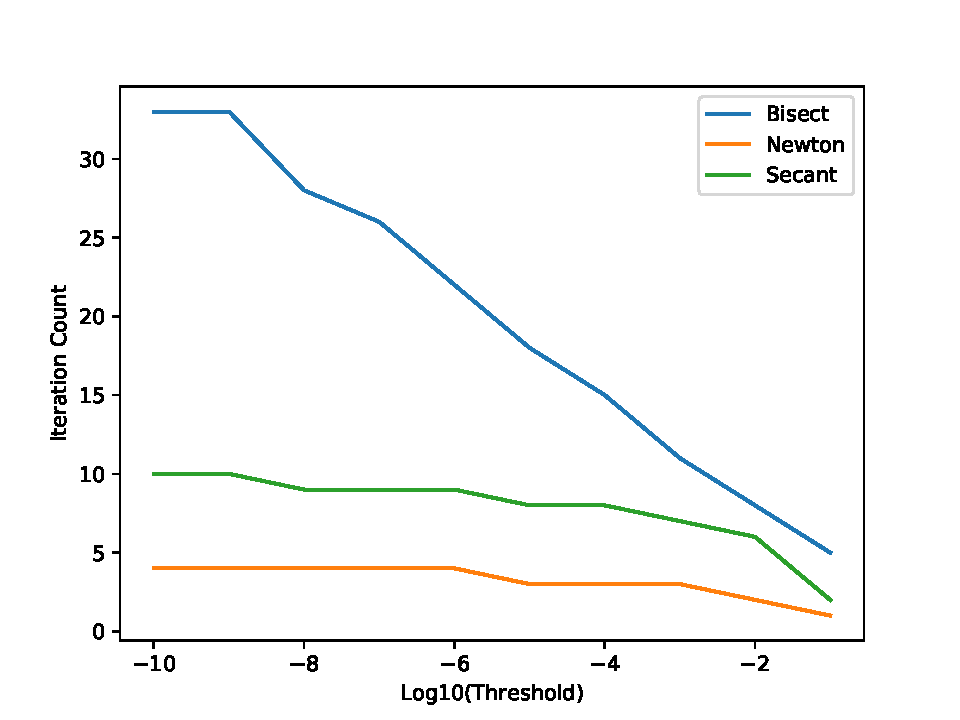
\includegraphics[width=5.5in]{Threshold_Count_Plot.pdf}}
      \caption{Plot of the iteration count versus threshold for the three methods of root finding used in this homework. It appears that the newton and secant methods are much more preferable, but they have limitations and use case restrictions when compared to the bisect method.}
\end{figure}

\begin{figure}[!h]
	\centering
	\noindent
	\makebox[\textwidth]{
      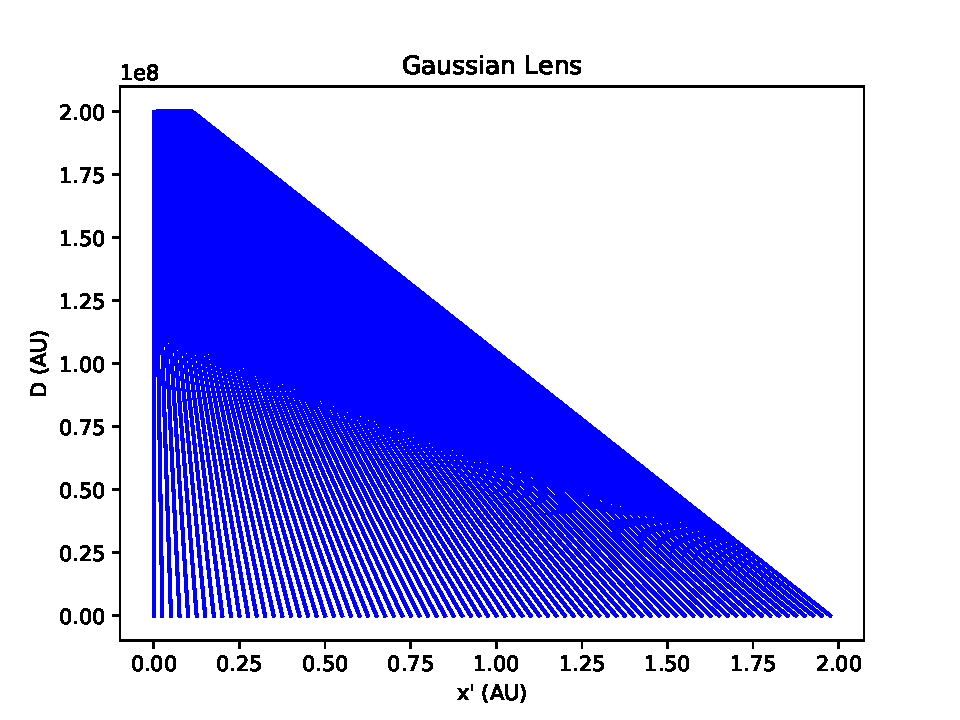
\includegraphics[width=5.5in]{GaussianLens.pdf}}
      \caption{Ray trace plot using a Gaussian lens model $x' = x\left[1+\frac{\lambda^2r_eN_0}{\pi a^2}e^{-\left(x/a\right)^2}\right]$ and solved using the bisect root find method. The rays appear to converge towards a point source, but the caustics are not visible at this resolution.}
\end{figure}

\begin{figure}[!h]
	\centering
	\noindent
	\makebox[\textwidth]{
      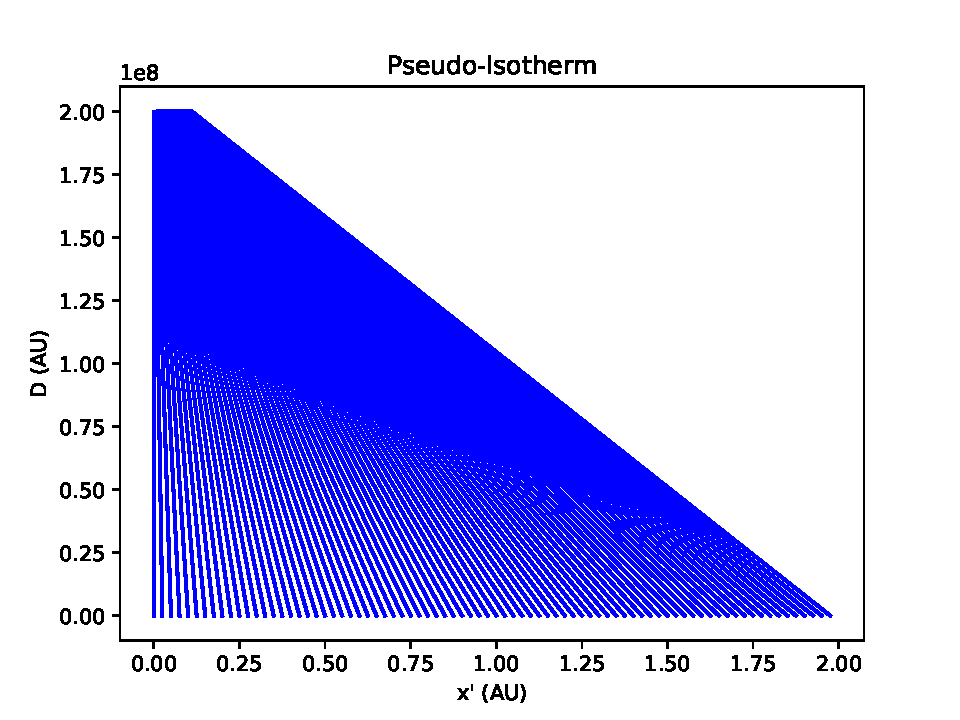
\includegraphics[width=5.5in]{PseudoIsotherm.pdf}}
      \caption{Ray trace plot using a pseudo-isotherm model $x' = x\left[1+\frac{\lambda^2r_eN_0}{\pi a^2}\left[1+\left(\frac{x}{r_c}\right)^2\right]^{-1/2}\right]$ and solved using the bisect root finding method. The rays appear to converge towards a point source, but the caustics are not visible at this resolution.}
\end{figure}

\end{document}